\documentclass[11pt]{article}

\usepackage[margin=0.5in]{geometry}
\usepackage{changepage}
\usepackage{hyperref}
\usepackage{graphicx}
\usepackage{amsmath}
\usepackage{xcolor}
\usepackage{xparse}

\def\labelitemi{\ensuremath{\triangleright}}
\renewcommand{\url}[1]{{\texttt{#1}}}
\renewcommand{\line}[2]{{\vspace{4pt} \large \noindent\textsc{#1} \hfill \small{#2}}\vspace{0pt}}

\newif\ifisleft
% \isleftfalse % by default

%%% Get an environment variable from latex. %%%
% Shamelessly stolen from https://tex.stackexchange.com/questions/62010/can-i-access-system-environment-variables-from-latex-for-instance-home
\ExplSyntaxOn

\NewDocumentCommand{\getenv}{om}
{
\sys_get_shell:nnN { kpsewhich ~ --var-value ~ #2 } { } \l_tmpa_tl
\tl_trim_spaces:N \l_tmpa_tl
\IfNoValueTF { #1 }
  {
  \tl_use:N \l_tmpa_tl
  }
  {
  \tl_set_eq:NN #1 \l_tmpa_tl
  }
}

\NewDocumentCommand{\strcmp}{mmmm}{
  \str_if_eq:eeTF{#1}{#2}
    { #3 }
    { #4 }
}

\ExplSyntaxOff

\begin{document}

  \setlength{\parindent}{0em}
  \pagestyle{empty}

  \getenv[\withpic]{WITHPIC}

  \begin{center}
  \noindent\begin{minipage}{0.66\textwidth}
    \begin{center}
      \huge Jacopo Philip Moretti
    \end{center}
    \textit{CS MS student at EPFL, with interests in theorem provers, formal verification, and languages, both natural and programming.}

    18.08.03 :: +41 76 730 67 19 :: Chemin des Triaudes, 4b, 1015 Ecublens
    \begin{center}
      \href{https://people.epfl.ch/jacopo.moretti}{\url{email}} :: \href{https://github.com/quartztz}{\url{github}} :: \href{https://quartztz.github.io}{\url{website}}
    \end{center}
  \end{minipage}
  \strcmp{\withpic}{true}{
    \begin{minipage}{0.25\textwidth}
      \begin{center}
        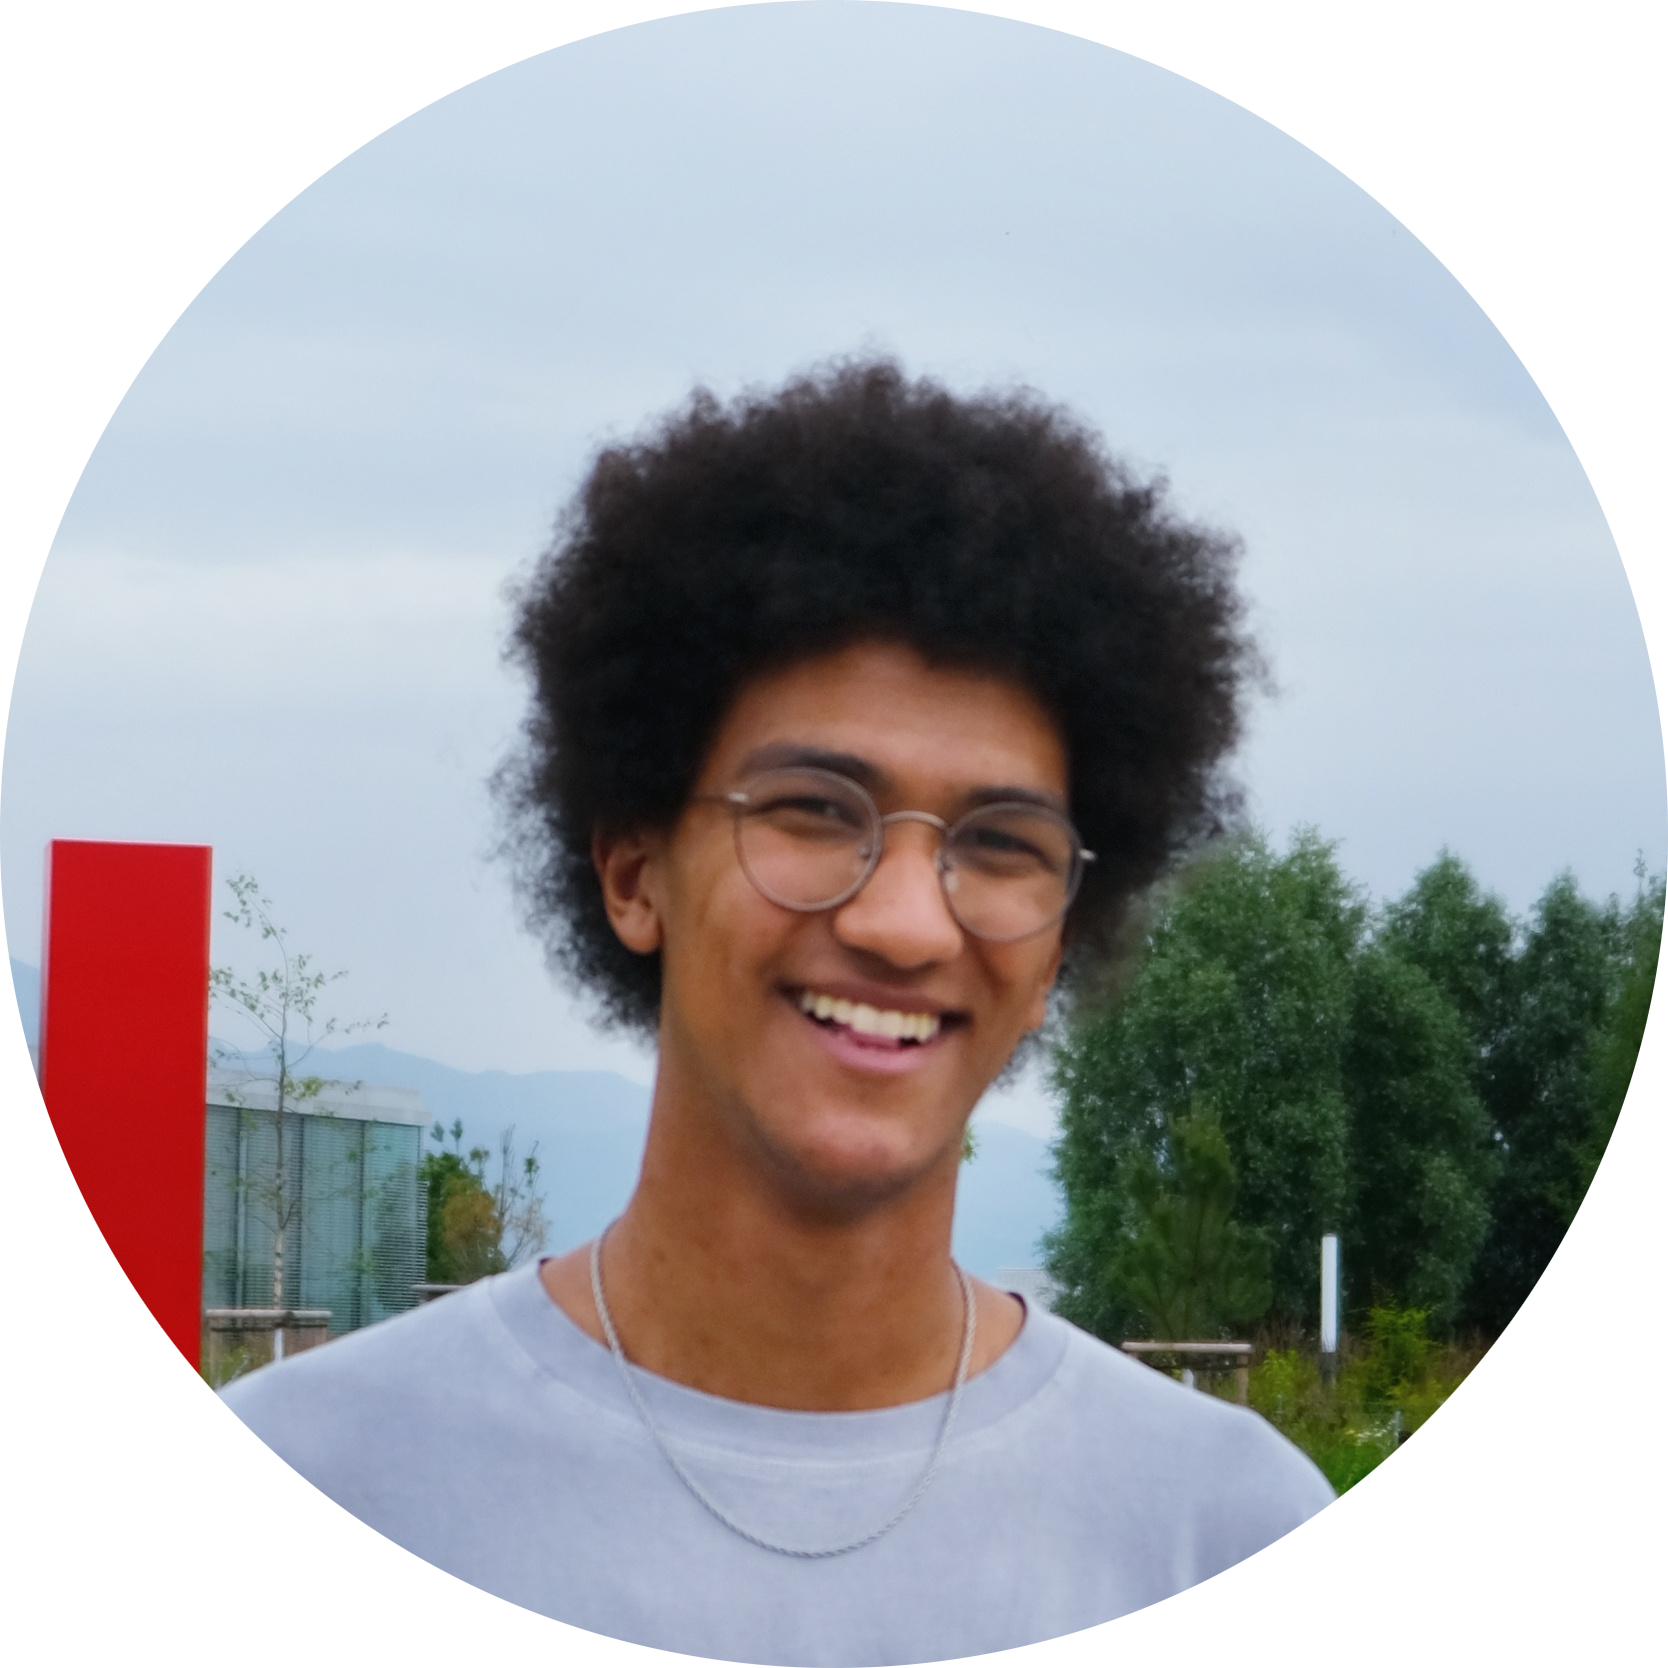
\includegraphics[width=.75\textwidth]{"./assets/img_circ.png"}
      \end{center}
    \end{minipage}
  }{
    % empty
  }
  \end{center}

  \subsection*{Academic}

  \line{MSc in Computer Science :: EPFL}{2024 - \textsc{Present}}

  Master's Degree in Computer Science at the \textit{Ecole Polytechnique Fédérale de Lausanne} (EPFL); projected end in 2026.

  \textbf{Specialization:} \textit{Foundations of Software}.

  \textbf{Fields of interest:} Theorem Proving, Programming Languages, Natural Language Processing.

  \textbf{Relevant courses:} \textit{Algorithms II (CS450), Machine Learning (CS433), Formal Verification (CS550)}.

  \vspace{0.75em}
  \line{BSc in Computer Science :: EPFL}{2021 - 2024}

  Bachelor's degree in Computer Science from the \textit{Ecole Polytechnique Fédérale de Lausanne} (EPFL).

  \textbf{Fields of interest:} Functional Programming, Programming Languages.

  \textbf{Relevant courses:} \textit{Algorithms (CS250), Functional Programming (CS207), Computer Language Processing (CS320), Logique Mathématique (MATH381), Software Enterprise (CS311)}.

\textbf{Awards:} \textit{1st place in the Battle of The Apps, prize awarded by Prof. Candea for the best project in the CS311 course (2023).}
  \subsection*{Experience}

  \line{Chief Product Officer :: actualia}{2024 - \textsc{Present}}

  CPO at \textit{actualia}, a startup creating a personalized press review app. Managed design team and led frontend development.

  \textbf{Skills:} \textit{Design (Figma), Android Mobile Development (Flutter, Dart, Bloc)}
  \vspace{0.75em}

  \line{Student Assistant :: Software Construction (CS214)}{FW 2023}

  Student Assistant for Profs. Odersky, Pit-Claudel, and Kunčak. Answered 100+ student queries on forums, explained concepts in class, and implemented a workflow for recording and editing 20+ course videos.

  \textbf{Skills:} \textit{Functional Programming (Scala), Video Editing (DaVinci Resolve), \emph{\texttt{git}}}
  \vspace{0.75em}

  \line{Student Assistant :: Students 4 Students}{2022, 2023}

  Volunteer at \textit{Students 4 Students}, developing classes and problem sets for Calculus, Linear Algebra, and Discrete Mathematics, and tutored during exercise sessions.
  \vspace{0.75em}

  \line{Technical Manager :: Fréquence Banane}{2022 - 2024}

  Committee member tasked with maintaining the technical (audiovisual and server) infrastructure of an 80+ member student radio. Gained knowledge in writing code for large scale and long term use, managing a technical team, and audio engineering.

  \textbf{Skills:} \textit{Python, VueJS, Astro}
  \subsection*{Skills}

  \begin{adjustwidth}{6em}{}
    \begin{itemize}
      \item[\textbf{Languages}] Italian (native), French (native), English (fluent), German (basic).
      \item[\textbf{Programming}] Scala, Java, Rust, C, Python, Dart, \{Java, Type\}Script.
      \item[\textbf{Design}] Adobe Suite, Figma.
    \end{itemize}
  \end{adjustwidth}

\end{document}
